% !Mode:: "TeX:UTF-8"
% !TEX program  = xelatex

% \documentclass{hfutreport}
\documentclass[bwprint]{hfutreport}

\title{基于以太坊的微博系统设计与实现}
\stunum{20184347, 2018xxxx}
\stuname{王\quad 浩, 李涵威}
\stuclass{信息安全2班, 信息安全1班}
\supervisor{叶春晓}
\dateinput{\today}

\begin{document}

\maketitle

% 目录使用Romen页脚 
\pagestyle{plain}
\pagenumbering{Roman}
\tableofcontents
\newpage
\pagestyle{plain}

%正文页脚
\setcounter{page}{1}
\pagenumbering{arabic}

\section{项目简介}
\subsection{概述}
这是一个运行在以太坊上的去中心微博系统,去中心化意味着没有一一个中心化机构能够控制你发送的微博,你
发送的微博是由你完全控制的,任何人无法删除、关闭你的微博。一旦你的微博发出去后,只有你自己能删除它。

\subsection{传统微博与去中心化微博的对比}
传统微博(如新浪微博)就是一个中心化的应用平台,新浪公司就是整个微博平台的中心。新浪公司制定新浪微博
的运行规则,开发出整个微博平台,为其提供中央服务器,维持着整个新浪微博的运转,并不断地向外推广,吸引
用户使用。一切商业行为都是为了追逐利益的,新浪公司运营新浪微博,也是为了吸引广告主投放广告,从而获得
巨额的广告收入。

在中心化的微博平台中,大致流程如\cref{fig:classical-weibo}~所示,博主(发微博者)会编辑微博发送到新浪微博平台中,新浪微博将微
博推送给观众(看微博者),观众查看微博,微博中会夹杂着一些广告,观众看微博时也会看到一些广告。广告主
会为广告的浏览量和点击量,支付广告费给新浪公司。

\begin{figure}[!htbp]
    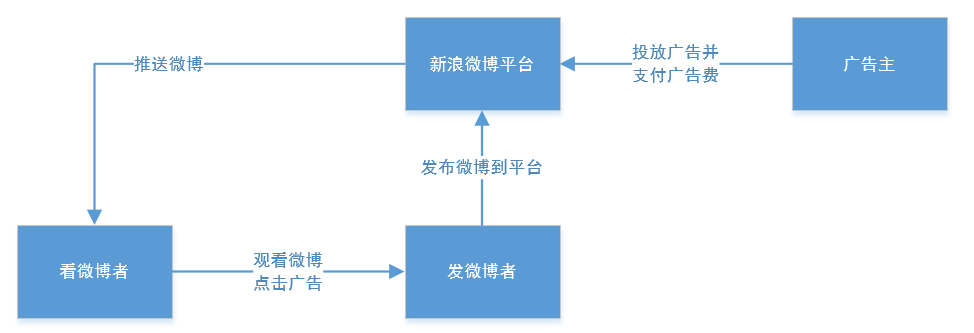
\includegraphics[width=\linewidth]{classical-weibo}
    \caption{传统中心化微博运作流程}
    \label{fig:classical-weibo}
\end{figure}

与传统微博平台不同,在去中心化微博平台中,将没有中心机构,没有中央服务器,主要是通过区块链技术,运用
分布式自治组织(DAO)的组织架构,实现微博平台的自治。让每一个微博参与者都成为微博平台的所有者,他们
将共享微博平台获得的全部收益。

\section{系统框架图(功能结构图)}


\section{功能说明}
本系统的核心业务围绕微博展开,其中用户可以发送微博,其他用户可以查看该微博并决定是否点赞或者点踩。
系统管理员可以查看所有用户信息,例如用户的微博总数、点赞总数、点踩总数等。

本系统主要涉及两类用户:微博用户和管理员。各用户的功能如\cref{tab:func}~所示。
\begin{table}[!htbp]
    \caption{用户功能}\label{tab:func}
    \centering
    \begin{tabular}{ccl}
        \hline
        \textbf{}                 & \textbf{需求要点} & \textbf{备注}                                        \\ \hline
        \multirow{5}{*}{微博用户} & 注册              & 使用以太坊账户注册一个微博账户,并指定一个唯一的昵称 \\
                                  & 登录              & 使用以太坊账户进行登录,一般由MetaMask自动完成       \\
                                  & 查询              & 用户查询自己的个人信息,包括ID、昵称、历史微博等     \\
                                  & 点赞              & 用户可以对首页看到的其他用户的微博进行点赞           \\
                                  & 点踩              & 用户可以对首页看到的其他用户的微博进行点踩           \\ \hline
        管理员                    & 查询              & 管理员可以查看完整的用户列表、微博总数等系统信息     \\ \hline
    \end{tabular}
\end{table}

可以看到我们的管理员出了查询系统信息外不具有其他功能,所以简单起见我们没有在系统中特别设立管理管,任何用户
都可以在后台页面查看后台信息和用户列表,也就是说目前所有用户其实都拥有和管理员一样的功能。

\section{设计思路}
\subsection{创建项目}
\subsection{合约}
\subsection{前端应用}

\section{结果展示}


\section{小组分工}
我们小组共两位成员,分工情况如\cref{tab:xzfg}~所示。另外我们在GitHub上进行项目合作,完整项目代码见
仓库\href{https://github.com/iamwhcn/dapp-weibo}{https://github.com/iamwhcn/dapp-weibo}。
\begin{table}[!htbp]
    \caption{小组分工}\label{tab:xzfg}
    \centering
    \begin{tabular}{c|c|l}
        \hline
        {\bf 姓名} & {\bf 学号} & {\bf 分工}         \\
        \hline
        王\quad 浩 & 20184347   & 系统设计、报告编写 \\
        \hline
        李涵威     & 2018xxxx   & 系统设计、报告编写 \\
        \hline
    \end{tabular}
\end{table}



\end{document}